% ============================================================================
% Complex Networks & Their Applications---Springer SVProc contribution
% ============================================================================
\documentclass{svproc}

\usepackage{graphicx}
\usepackage{multirow}
\usepackage{amsmath,amssymb,amsfonts}
\usepackage{mathrsfs}
\usepackage{xcolor}
\usepackage{textcomp}
\usepackage{manyfoot}
\usepackage{booktabs}
\usepackage{algorithm}
\usepackage{algorithmicx}
\usepackage{algpseudocode}
\usepackage{tikz}
\usetikzlibrary{arrows.meta,positioning}
\usepackage{url}
\renewcommand{\floatpagefraction}{0.85}
\renewcommand{\topfraction}{0.9}
\renewcommand{\textfraction}{0.08}
\def\UrlFont{\rmfamily}
\def\orcidID#1{\unskip$^{[#1]}$}

% Drafting aid---must be unused at submission time.
\newcommand{\TODO}[1]{\textcolor{red}{[TODO: #1]}}
% Numeric placeholder---data from the 2026-07-22 rebuild run
% (experiments/aqueducts/final_benchmark.csv) to be filled in. Every \dtba MUST be
% resolved before submission. Optional arg = a hint of what number goes there.
\newcommand{\dtba}[1][?]{\textcolor{red}{\textbf{[#1]}}}

% Notation used throughout (Sec. 3): keep consistent, define once.
\newcommand{\worstof}{\mathrm{worst\_of}}
\newcommand{\bestof}{\mathrm{best\_of}}

\newcommand{\enginepanel}[3][0.7\textwidth]{%
  {\scriptsize #2}\\[1pt]\includegraphics[width=#1]{#3}}
\definecolor{cascgreen}{HTML}{22C55E}
\definecolor{cascred}{HTML}{EF4444}
\definecolor{cascring}{HTML}{FBBF24}
\definecolor{casclbl}{HTML}{52525B}
\newcommand{\legdia}[1]{\tikz[baseline=-0.7ex]{\fill[#1] (-2.4mm,0)--(0,2.4mm)--(2.4mm,0)--(0,-2.4mm)--cycle;}}
\newcommand{\legoct}[1]{\tikz[baseline=-0.7ex]{\fill[#1] (22.5:2.6mm) \foreach \a in {67.5,112.5,157.5,202.5,247.5,292.5,337.5}{--(\a:2.6mm)}--cycle;}}
\newcommand{\legcir}[1]{\tikz[baseline=-0.7ex]{\fill[#1] (0,0) circle (2.2mm);}}
\newcommand{\legcrack}{\tikz[baseline=-0.7ex]{\fill[cascred] (0,0) circle (2.2mm);
  \draw[white,line width=.7pt] (-0.6mm,2.1mm)--(0.4mm,0.4mm)--(-0.5mm,-0.3mm)--(0.5mm,-2.1mm);}}
\newcommand{\legring}{\tikz[baseline=-0.7ex]{\draw[cascring,line width=.9pt] (0,0) circle (2.6mm);\fill[cascgreen] (0,0) circle (1.7mm);}}
% Category glyphs cropped straight out of fig_office_blackout.png (black strokes
% on transparency), so the legend shows the very icons the screenshots use.
\newcommand{\legicon}[1]{\raisebox{-0.55ex}{\includegraphics[height=2.5mm]{#1}}}
\usepackage[hidelinks]{hyperref}
\urlstyle{same}   % keep URLs in the body font rather than typewriter

\begin{document}
\mainmatter 

\title{Composable, Knowledge-Driven Disservice Propagation for Complex Interdependent Services with a Flow-Allocation Module Validated Against Hydraulic Simulation}

\titlerunning{Composable Knowledge-Driven Disservice Propagation}

\author{Cristian Curaba \and Stefano Grimaz}
\authorrunning{C. Curaba and S. Grimaz}
\institute{University of Udine, Udine, Italy,\\
\email{cristian.curaba@uniud.it}}

\maketitle

\begin{abstract}
% Springer SVProc guide (instructions_for_authors.pdf, p.4): abstract 150-250
% Page count: 12 pp
Modeling cascading failure across interdependent critical infrastructure requires either
a composable physical simulator per domain or a topological abstraction that discards
quantity awareness. Simulators are costly, data-hungry, and needs detailed calibration per domain; topological
abstractions stay data-parsimonious while missing quantity-based behaviors that govern real dynamics. 
We present, instead, a knowledge-driven propagation architecture in which heterogeneous
service dependencies are identified by categories: a general logical propagation resolves
multi-dependency and redundancy structures purely from how nodes are categorized, while
quantity-aware categories plug in dedicated mechanisms---here, a max-min fair-share flow
module for water distribution. Both share one discrete functionality scale and a
monotonic update algorithm guaranteeing convergence in finitely many rounds. 
We assess the flow module by comparing its results with those we get from preexisting
pressure-driven WNTR simulation on eight realistic networks across four failure families (clustered damage, capacity-targeted attack, source failure,
tank loss). Under capacity-targeted attack and source failure a topological-reachability baseline misses
46\% of the truly critical junctions, where the flow module misses 10\% and 8\% at an average critical-class precision of
0.73.\footnote{Supplementary materials, code and results are available at:
\url{https://github.com/cascade-platform-org/CASCADE}. The platform itself runs at \url{https://app.cascade-platform.org/}.}
\keywords{cascading failures, interdependent networks, critical infrastructure, water distribution networks, network flows}
\end{abstract}

% ============================================================================
\section{Introduction}\label{sec:intro}

Hazards frequently trigger cascading failures across interdependent
critical infrastructure, amplifying initial damage well beyond the
footprint of the initiating event---from Hurricane Maria's long-lasting
multi-system service crisis in Puerto Rico~\cite{hurricane_maria} to the
April 2025 Iberian blackout's national-scale propagation into transport
and digital services~\cite{panel2025grid}. The UNDRR's resilient-infrastructure handbook
calls for tools that capture ``the interdependent nature of infrastructure and services
[\ldots] and the cascading impacts''~\cite{UNDRR2023Handbook}.

Existing computational approaches sit at two extremes. Physical simulators reproduce one
domain's dynamics with high fidelity, at the price of extensive domain-specific
calibration that does not apply to another domain's physics. Topological and
network-of-networks models generalize across domains on structural information alone, while
discarding the quantity-aware dynamics---partial supply, congestion, priority-driven
allocation---that decide whether a service is actually delivered.

One system needs both readings, for different dependencies. Whether a district still
has water is a question of \emph{how much}: a limited supply divides across contended
mains. Whether its pumping station still runs is a question of \emph{whether}: it needs
electricity and telemetry which generally are either available or not. No framework we know of
resolves both kinds inside a single architecture that a domain expert extends by
declaring just a few node attributes, rather than by writing/integrating a new solver for each kind of
dependency.

This paper presents such an architecture. Its core node attribute is the
\emph{category}: a named service---water, electricity, digital---that the node provides.
Every element carries a \emph{functionality} on a small
discrete scale running from fully operational down to complete loss.
Every category is resolved the same logical way: a node needs all the categories it
depends on while within one category a single healthy supplier suffices, which is how redundancy is expressed.
A category is \emph{additionally} passed to the quantity-aware mechanism when its resource is consumed
in measurable amounts, where a max-min fair-share allocation divides the available supply
among node consumers, bounded by edge capacities.

The propagation algorithms meet on one scale and commit through one rule: a commit
can only hold or lower an element's functionality, never raise it. The iteration
therefore cannot cycle and terminates on any topology, whichever mechanism produced the
proposal.

Of the two mechanisms, only the quantity-aware one has an independent physical simulator
to check it against, and that is what we validate in Section~\ref{sec:validation}: 
the flow module (labelled with information gained from the simulation itself) against
pressure-driven hydraulic simulation of the same failures on the same networks.
We highlight that the module's scope is to allow a practitioner to rapidly emulate the effects of a failure on a water network
without having all the physical parameters that a full hydraulic simulation would require.
The module is not intended to replace detailed hydraulic analysis but to provide a fast, 
approximate assessment of the network's resilience under various failure scenarios.
The validation shows that the flow module is able to capture the hydraulic behavior of water networks with high fidelity
by exploting few informations gained from the EPANET file (the input data) and the hydraulic simulation only to fix edge orientations.

\paragraph{Contributions.} (1) A composable, category-based propagation
architecture in which quantity-aware and purely logical interdependencies
share a single convergent update rule (Section~\ref{sec:architecture}). 
(2) A pipeline to automatically label node and edge attributes exploting information gained from hydraulic
solutions (Section~\ref{sec:importer}). (3) A validation of that module against
independent pressure-driven simulation on eight networks (Section~\ref{sec:validation}).
% ============================================================================
\section{Related Work}\label{sec:related}

Foundational work on interdependent infrastructure established the
classification of interdependencies into physical, cyber, geographic, and
logical dimensions~\cite{rinaldi_identifying_2002}; the
modeling-and-simulation literature that followed spans empirical,
agent-based, economic, and network-based
approaches~\cite{ouyang_review_2014}. Subsequent network-of-networks
research showed that even weak inter-system coupling
can trigger abrupt, catastrophic collapse rather than gradual degradation
\cite{buldyrev_catastrophic_2010,gao_networks_2011}.
These studies characterize \emph{when} cascades occur but stop short of a
computational mechanism a practitioner can run on an arbitrary network; our
logical propagation operationalizes exactly that. In
multilayer-network terms~\cite{kivela_multilayer_2014,boccaletti_structure_2014},
our categories play the role of layers to model the disservice propagation across them.


Networks are far more vulnerable to targeted removal of their most important elements than
to random loss~\cite{albert_error_2000} which is the regime that matters for
resilience assessment, and the harder one to predict. Three of our four failure
families are deterministic attacks of that kind, aimed at main pipes and pumps and at storage (Section~\ref{sec:validation}).

Load-redistribution models~\cite{motter_cascade-based_2002,crucitti_model_2004} treat a
different mechanism: losing one element reroutes its load onto others, and where
that load exceeds a survivor's capacity the survivor fails in turn---modelled
for water distribution~\cite{shuang_performance_2014} and for
interdependent water--power systems~\cite{li_cascading_2025}. Our module
allocates capacitated flow against demand declared at explicit sources, so a
shortfall surfaces as unmet delivered quantity (Section~\ref{sec:discussion}).
Network-flow formulations of interdependent infrastructure are well established for service
restoration~\cite{lee_restoration_2007}, and broader resilience
reviews~\cite{de_marco_quantitative_2025,hines_topological_2010} converge on the
gap this paper addresses: topological metrics are data-parsimonious but
function-blind, while performance-based models capture function at the cost of
per-domain simulation machinery with no practical way of doing comprehensive evaluations.

For water-network tooling, WNTR~\cite{klise_software_2017} implements the
pressure-driven demand (PDD) formulation~\cite{wagner_water_1988} we use
as ground truth (Section~\ref{sec:validation}); our importer's optional
node-budget reduction uses its skeletonization by diameter
threshold~\cite{saldarriaga_water_2012}. EPANET~\cite{rossman2000epanet}
is the solver both are built on. Graph-theoretic robustness measures for water
networks~\cite{yazdani_complex_2011,herrera_graph_2016} are the closest
precedent for our reachability baseline: they judge a network from its topology
alone, which costs nothing to compute but says nothing about how much water is
actually delivered. How well they predict has been shown to depend on where the
sources sit~\cite{meng_topological_2018}. Machine-learned
surrogates~\cite{garzon_machine_2022} occupy the same niche from the
opposite direction---capturing hydraulics but needing per-network
training data, where our flow module is built from
one import of the network file itself. Our flow module's
allocation builds on classical max-min fairness
principle~\cite{nace_tutorial_2006} standard in network resource
allocation, implemented via NetworkX~\cite{hagberg_exploring_2008}.

% ============================================================================
\section{The Propagation Architecture}\label{sec:architecture}

We introduce the architecture through one small example
(Section~\ref{sec:arch-example}), then make each of its parts precise: the elements a
model is built from and how their categories are typed
(Section~\ref{sec:arch-model}), the logical propagation (Section~\ref{sec:arch-logical}) and the flow module
(Section~\ref{sec:arch-flow}), and finally the shared update rule that composes them
and guarantees convergence (Section~\ref{sec:arch-pipeline}).

\subsection{Running Example: An Office}\label{sec:arch-example}

Figure~\ref{fig:example} shows an office with common dependencies: the served office node depending on two \textsc{SourceToDemands} categories---\emph{electric} (an \textsc{Electrical Source} feeding an
\textsc{Electrical Infrastructure}) and \emph{heat} (a \textsc{Gas Source} feeding
a \textsc{Heater Generator})---and one \textsc{Requisite} category, \textsc{digital},
through two independent devices, a \textsc{Laptop} and an \textsc{Office PC}.

\emph{Redundancy vs Requirements.} Losing either digital device alone leaves the
office's digital dependency intact, one surviving device being enough; the
logical propagation encodes this by aggregating the functionality of
parent nodes (predecessors, joined by an edge oriented towards the node) within a
category via \emph{best-of}
(Section~\ref{sec:arch-logical}). The office, however, requires electricity,
heat, \emph{and} digital service together, which is \emph{worst-of} aggregation
across categories.

\emph{Quantity.} What the logical propagation leaves out is amount: whether a
source can cover every downstream demand concurrently. That is what
Section~\ref{sec:arch-flow}'s flow module supplies, and why
\textsc{SourceToDemands} categories route through it as well. The example is
deliberately minimal---one source per resource, no alternative routing---so
the flow module adds no behaviour here. Amount becomes decisive on a
\emph{capacitated} network with \emph{several} source-to-demand paths, the regime
the water networks of Section~\ref{sec:validation} exercise.


\begin{figure}[!t]
\centering
\begin{minipage}[b]{0.44\textwidth}\centering
{\scriptsize (a) after the blackout event}\\[1pt]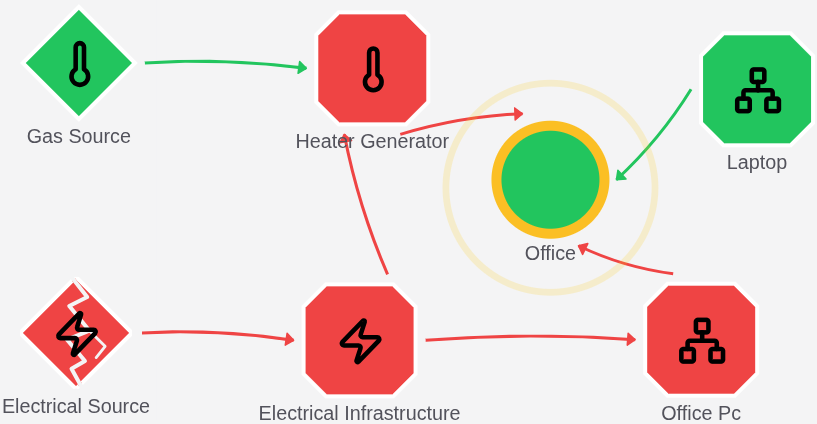
\includegraphics[width=\linewidth]{fig_office_blackout}
\end{minipage}\hfill
\begin{minipage}[b]{0.44\textwidth}\centering
{\scriptsize (b) under a shared digital fault}\\[1pt]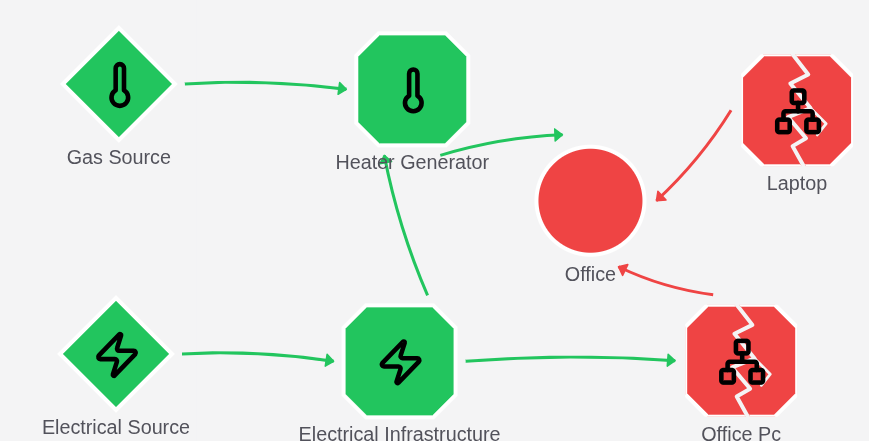
\includegraphics[width=\linewidth]{fig_office_digital}
\end{minipage}

\vspace{3pt}
{\centering\scriptsize
\legdia{casclbl!55}\,Source \quad
\legoct{casclbl!55}\,Infrastructure \quad
\legcir{casclbl!55}\,Service\\[2pt]
\legcir{cascgreen}\,operational \quad
\legcir{cascred}\,critical \quad
\legcrack\,struck by the event \quad
\legring\,backup defers the drop\\[2pt]
\legicon{icon_electric}\,\emph{electric} \quad
\legicon{icon_heat}\,\emph{heat} \quad
\legicon{icon_digital}\,\emph{digital}\par}
\vspace{3pt}

\caption{The running example as direct screenshots, both starting from a
baseline in which every node is operational. In~(a) the cracked Electrical Source zeroes the electric supply, so the Office~PC
shuts down and the Heater Generator drops by \emph{worst-of} across categories
(gas alone cannot run it). The Office itself stays functional, for two distinct
reasons: \emph{best-of} keeps its digital dependency alive through the surviving
Laptop, and its heat backup defers the drop for as long as the room stays warm
(yellow ring). In~(b) a shared software fault instead takes \emph{both} digital
devices critical: \emph{best-of} now has no surviving digital parent, and the
Office goes critical}\label{fig:example}
\end{figure}



\subsection{Elements, Functionality, and Category Typing}\label{sec:arch-model}

A modeled network is a directed graph, with nodes and edges each carrying an integer \emph{functionality} on a discrete scale
$1,\ldots,N$ ($1$ = complete loss, $N$ = full operation); small discrete
state scales are standard in disaster-loss modeling (e.g.\ Hazus damage
states~\cite{kircher_hazus_2006}), and $N$ is a modeling choice (defaulting to 3).
Every node is attributed with a set of \emph{categories}---named services such as
\emph{water}, \emph{electric}, or \emph{digital}---which represent the service it provides (generally, just one)
 and every category is \emph{typed}, which selects how that dependency is propagated.

Two algorithms do the propagating. The \emph{logical} propagation runs
for every node over all of its incoming edges as defined in
Section~\ref{sec:arch-logical}. A category typed \textsc{Requisite} is resolved by it
and nothing else. A category typed \textsc{SourceToDemands} triggers the flow module,
 which solves one capacitated allocation over the subgraph carrying
that category (Section~\ref{sec:arch-flow}). A node holding a proposal from both then
takes the worse of the two (Section~\ref{sec:arch-pipeline}).

Neither algorithm sets a functionality directly: each \emph{proposes} one, and per-node
attributes may adjust that proposal before it is committed. A category's
\emph{dependency level} attenuates how hard a drop in that category hits the node, and
a \emph{backup} defers the drop by a specified amount of time (as \textsc{Office} in
Figure~\ref{fig:example}). These guards and the commit that follows them are the subject
of Section~\ref{sec:arch-pipeline}.



\subsection{Logical Propagation}\label{sec:arch-logical}

For a target node $v$ with incoming edges $E_{\mathrm{in}}(v)$, let $(u\!\to\!v)\in E_{\mathrm{in}}(v)$ be one such
edge, $u$ its parent node, $s(u)\in\{1,\ldots,N\}$ that parent's functionality and
$s(u\!\to\!v)$ the edge's own. The logical propagation adopts two primitive combinators
on the totally ordered scale: $\worstof(x,y)=\min(x,y)$, modeling \emph{requirement}
(every input must hold for the output to hold), and $\bestof(x,y)=\max(x,y)$, modeling
\emph{redundancy} (one healthy input in the same category suffices). Three steps form
it, each a deterministic function of the parent nodes' and edges' functionalities:
\begin{enumerate}
  \item \textbf{Deliverable functionality}---a degraded parent and a
    degraded connecting edge both limit what can reach $v$:
    $L(u\!\to\!v)=\worstof\big(s(u),\,s(u\!\to\!v)\big)$.
  \item \textbf{Intracategorical aggregation}---within one category $g$,
    one healthy supplier is enough:
    $C_g(v)=\bestof\big\{L(u\!\to\!v):(u\!\to\!v)\in E_{\mathrm{in}}^g(v)\big\}$, 
    where $E_{\mathrm{in}}^g(v)\subseteq E_{\mathrm{in}}(v)$ are the incoming edges whose parent supplies category $g$.
  \item \textbf{Intercategorical aggregation}---$v$ requires \emph{every}
    category it depends on, so categories combine by requirement:
    $s^{\mathrm{logic}}(v)=\worstof\big\{C_g(v):g\in G(v)\big\}$, with $G(v)$ the
    categories represented among $v$'s parents.
\end{enumerate}

The two combinators are the many-valued generalization of classical fault-tree
\textsc{and}/\textsc{or} gates~\cite{vesely1981fault}: a node's proposal is a
deterministic function of its parents' functionality with no free parameter, computable
by inspection on the running example.

\subsection{Capacity-Based Propagation: A Plug-In Flow Module}\label{sec:arch-flow}

A \textsc{SourceToDemands} category says that a resource is sourced, carried and
consumed in continuous amounts. It does not say how that resource should be divided
when there is not enough of it, and the answer depends on what is being emulated: a
water distribution system redistributes by physical law, a supply chain by contract.
This section describes the flow module whose fidelity Section~\ref{sec:validation}
measures against hydraulic simulation.

For a typed \textsc{SourceToDemands} category, the module extracts the induced subgraph
and solves one priority-aware capacitated flow problem on it. Within that subgraph,
\emph{source} nodes supply the resource at a rate scaled linearly by their own
functionality, \emph{infrastructure} nodes relay it under a throughput capacity, and
\emph{service} nodes only consume it, while edges carry a capacity; every one of these
limits is scaled by the element's functionality. The module solves this on an auxiliary
directed graph. Every node is split into an \emph{in} and an \emph{out} vertex joined by
an edge carrying that node's throughput, so a node's own capacity is enforced like any
other edge capacity, and the original edges run from one node's \emph{out} vertex to the next
node's \emph{in} vertex. A super-source feeds each supplying node at its effective
supply, and each demanding node drains into a super-sink at its declared demand. It allocates flow across this
graph by \emph{priority-tiered max-min fairness}~\cite{nace_tutorial_2006}: higher tiers
served fully first, equal-priority consumers sharing any shortage as evenly as
the network physically allows (max-min water-filling by repeated max-flow with a
residual-reachability bottleneck test). For each consuming node, the delivered
fraction $r$ of declared demand quantizes to a proposed functionality
$s^{\mathrm{cap}}(v)=\max(1,\lceil r N\rceil)$. 
Priority is a \emph{modelling} input---``serve $X$ before $Y$'' from expert knowledge of how the system is actually
operated.

\subsection{Shared Update Rule and Convergence}\label{sec:arch-pipeline}

Every round applies the same three steps to every node---\emph{propose},
\emph{guard}, \emph{commit}---whichever propagation is involved.

\emph{Propose.} Section~\ref{sec:arch-logical} yields $s^{\mathrm{logic}}(v)$ for every
node, and Section~\ref{sec:arch-flow} yields $s^{\mathrm{cap}}(v)$ for each node
with a \textsc{SourceToDemands} category. Both live on the same $1,\ldots,N$
scale, so a node holding both aggregates them by necessity,
$s^{\mathrm{prop}}(v)=\worstof\big(s^{\mathrm{logic}}(v),\,s^{\mathrm{cap}}(v)\big)$,
while a node holding only one takes it unchanged.

\emph{Guard.} Two per-category attributes may then soften that proposal, carrying
$s^{\mathrm{prop}}(v)$ into the guarded value $s^{\mathrm{guarded}}(v)$ the commit
consumes. A guard only modulates a drop the mechanisms have already proposed,
and a node that declares nothing gets the worst case (representing full dependency and no
reserve). The \emph{dependency level} $d\in\{1,\ldots,N\}$ states how hard the node
leans on a category, attenuating a proposed level $\ell$ to $\min(N,\,\ell+(N-d))$: at
$d=N$ the drop passes in full, at $d=1$ it is neutralized, and values between reduce it
linearly. A \emph{backup} then defers whatever survives attenuation: a node with a declared reserve
in the dropping category holds its functionality and starts a countdown of that
reserve's duration, so the drop lands only when the reserve expires. A backup covers its
own category alone, so a simultaneous drop through an unbacked category still commits
this round.

\emph{Commit.} The guarded proposal is committed monotonically:
\[
  s^{\mathrm{new}}(v) = \worstof\big(s^{\mathrm{old}}(v),\, s^{\mathrm{guarded}}(v)\big).
\]
Functionality can therefore only hold or worsen, never improve. This single inequality
is what guarantees convergence.
Every round lowers at least one element by at least one level until convergence is reached, and
the total descent available across the model is $(N-1)(|V|+|E|)$, so the iteration
terminates after at most $(N-1)(|V|+|E|)+1$ rounds whatever the topology and attributes---in
practice far sooner, since a round updates every element in parallel.

% ============================================================================
\section{Building the Flow Module from Data: The EPANET Importer}\label{sec:importer}

Water utilities exchange networks as EPANET \texttt{.inp} files, which carry the
physical detail of the aqueduct infrastructure. We wrote a pipeline that reads
such a file and produces a categorized node/edge model with no manual step. Four
decisions carry the module's fidelity; Supp.~Mat.~S1 specifies every stage in full.

\emph{What becomes a source, and how much it supplies.} An EPANET file distinguishes two kinds
of water body: a \emph{reservoir} is large enough to treat as inexhaustible while a \emph{tank} is a
finite store, capped at the rate it is seen delivering while the network is intact.
Consuming junctions become nodes with reported demand. Pumps and valves
become inline \textsc{Requisite}-category nodes, so a stopped pump gates everything downstream
through the logical propagation rather than through device-specific code. Pipes become
capacitated directed edges, and demand is read at the busiest hour of the day.

\emph{Which way the edges point.} A file records one direction per pipe, but that is
only the direction in the operating state the file describes; elsewhere in the day, or
after a failure, water can run the other way. We recover direction from behaviour
instead through various \emph{hydraulic} solutions---raising demand, and
closing one link at a time---and we read each pipe's direction from the sign of its
simulated flow. A pipe seen flowing both ways
becomes two opposed directed edges, as does one whose only observed flow is too slow to
trust: committing to a direction that is solver noise can silently cut off
everything downstream.

\emph{How much each pipe carries.} A file gives a pipe's diameter but not its capacity.
We apply one design velocity to every pipe, $v_{\text{design}}=2.5$\,m/s, the standard
figure for water mains, so a pipe of diameter $d$ carries
$\tfrac{\pi}{4}d^2 v_{\text{design}}$. Finer per-pipe assumptions do not improve fidelity (Supp.~Mat.~S5).

\emph{Who gets water first is left unset.} Deriving that ordering from the network's own
behaviour under failure gave no fidelity gain (Supp.~Mat.~S7), so the importer assigns
none and every number in Section~\ref{sec:validation} uses a flat allocation, equal
consumers sharing a shortage evenly. Priority remains central to \emph{authoring}. An
expert who knows how a utility distributes water states that knowledge in one attribute
per node. Where valve control makes the ordering a real operational choice, the same
attribute serves a second purpose: comparing competing policies under shortage
(Section~\ref{sec:discussion}).

% ============================================================================
\section{Module Validation Against Hydraulic Simulation}\label{sec:validation}

This section validates the flow module's fidelity to real hydraulics: the importer builds
the module from EPANET files, and its output is compared to a pressure-driven WNTR solutions
on the same network.

\emph{Validation Protocol.} For each of eight networks (three textbook WNTR examples
(Net1, Net2, Net3), three real, anonymized Italian aqueducts, and two the public
 Modena and C-Town \cite{kentucky_water_resources_research_institute_university_of_kentucky_water_nodate})
we generate structural-failure situations,
apply the identical intervention to a pressure-driven (PDD) WNTR solve and to
the imported model, and compare per-junction functionality. Both sides take
demand at the coincident system peak (Section~\ref{sec:importer}). We report three
quantities. The \emph{Functionality Match Score} (FMS) measures agreement on
\emph{how much} service each junction retains. Fix one situation, and let $J$ be its
demand-bearing junctions, each $j \in J$ carrying declared demand $d_j$ and $\ell^{\mathrm{WNTR}}_j$, $\ell^{\mathrm{module}}_j$
respectively the functionality levels (linearly mapped fraction of the demand satisfied) of the WNTR solve and the module,
 both in $\{1,\ldots,N\}$. Then
\[
  \mathrm{FMS} \;=\; 1 \;-\; \sum_{j \in J} w_j\,
  \frac{\bigl|\ell^{\mathrm{WNTR}}_j - \ell^{\mathrm{module}}_j\bigr|}{N-1},
  \qquad w_j = \frac{d_j}{\sum_{k \in J} d_k}.
\]
Each junction contributes its level disagreement, divided by $N-1$, the largest the functionality scale
allows, and weighted by $w_j$, its share of the situation's demand. FMS is $1$ on exact
agreement and $0$ when the two sides differ by the full scale on every unit of demand.

We evaluate at $N=3$ (critical / degraded / operational), the coarsest scale that still
separates partial from total service loss. Agreement moves by less than 0.005 across functionality scale sizes and service-pressure conventions (Supp. Mat. S6).

The second and third quantities look only at the \emph{critical} class, level $1$,
against everything above it. For one situation let $W$ be the junctions the WNTR
solve reports critical and $M$ those the module flags. Then
\[
  \mathrm{precision} = \frac{|M \cap W|}{|M|},
  \qquad
  \mathrm{recall} = \frac{|M \cap W|}{|W|}.
\]
Recall asks what share of the genuinely critical junctions were found by the module; precision asks
what share of the module's critical flags were real. Both are computed \emph{per situation} and then
averaged over situations. A
fifth of our situations are ones in which the network's redundancy absorbs the
disruption entirely, leaving $W$ empty; a model that correctly flags nothing scores
recall $1$ there. Symmetrically a model that flags nothing at all,
$M$ empty, scores precision $1$.

For conservative resilience analysis recall is the
metric that matters most. We score two baselines on the identical junction set: a
\emph{null model} predicting every junction fully operational, and a \emph{reachability
baseline}---the field's standard connectivity
abstraction~\cite{hines_topological_2010}---predicting a junction critical iff no
undirected path of in-service links connects it to a surviving source. 

We test four failure families, each a set of simultaneous element closures (one, two or
three at a time, capped $\sim\!60$ situations per family): \emph{cluster}, breaks within
two topological hops of a random epicentre (local hazard);
\emph{targeted}, among the largest-diameter mains and pumps (top fifth); \emph{source},
closing a reservoir's outlet; and \emph{tank}, closing every link on a tank. A closed
link carries zero flow. Table~\ref{tab:familydetect} pools the four
families over networks and seeds; Supp.~Mat.~S4 breaks them down per network and
Supp.~Mat.~S2 gives the complete protocol.

\emph{FMS: the baselines nearly saturate it.} Because most sampled
situations perturb only small parts of the network, raw FMS carries a strong ceiling
effect---the null model alone scores 0.82. Pooled across the four families the
module's level agreement is 0.92, reaching 0.97 on the mildest family
(Table~\ref{tab:familydetect}).

\emph{Recall: where quantity-awareness matters
(Table~\ref{tab:familydetect}).} Reachability is blind to any service loss short of
disconnection: under \emph{capacity-targeted attack} it misses 46\% of the truly
critical junctions where the module misses only 10\%, and it misses as many again
under \emph{source failure}---survivors stay connected but cannot push the lost
reservoir's yield through the surviving pipes, so reachability recovers just $0.54$
against the module's $0.92$, even though it is fully precise (always $1.00$) by
construction. The module holds recall at $0.90$--$0.98$ in every family, paying for
it in precision (0.73 on average, Table~\ref{tab:familydetect}) via over-warning.


\begin{table}[t]
\centering
\caption{The flow module against two baselines over all eight networks. Every score is a
mean over situations, each counting once, and the \textbf{average} row is the
$n$-weighted mean of the four family rows. \emph{crit.} is the share of scored junctions
that are truly critical. FMS is demand-weighted agreement with WNTR on \emph{how much}
service each junction keeps ($1$ = exact). Reachability scores precision $1.00$ by
construction: it calls a junction critical only when nothing connects it to a source, and
such a junction cannot be served. Families are defined in
Section~\ref{sec:validation}; the per-network breakdown is in Supp.~Mat.~S4}\label{tab:familydetect}
\setlength{\tabcolsep}{4pt}\small
\begin{tabular}{@{}lrr@{\hskip 1.1em}ccc@{\hskip 1.1em}cc@{\hskip 1.1em}cc@{}}
\toprule
 & & & \multicolumn{3}{c}{Mean FMS} & \multicolumn{2}{c}{precision} & \multicolumn{2}{c}{recall}\\
\cmidrule(lr){4-6}\cmidrule(lr){7-8}\cmidrule(l){9-10}
Family & $n$ & crit. & module & null & reach. & module & reach. & module & reach.\\
\midrule
cluster  & 459 & $3.9\%$  & 0.97 & 0.87 & 0.97 & 0.84 & 1.00 & 0.98 & 0.93\\
targeted & 384 & $30.9\%$ & 0.87 & 0.74 & 0.85 & 0.71 & 1.00 & 0.90 & 0.54\\
source   &  24 & $37.2\%$ & 0.78 & 0.65 & 0.73 & 0.51 & 1.00 & 0.92 & 0.54\\
tank     &  72 & $4.2\%$  & 0.87 & 0.95 & 0.98 & 0.20 & 1.00 & 0.94 & 0.92\\
\midrule
\textbf{average} & \textbf{939} & $16.1\%$ & \textbf{0.92} & 0.82 & \textbf{0.92} & 0.73 & \textbf{1.00} & \textbf{0.94} & 0.76\\
\bottomrule
\end{tabular}
\end{table}

% ============================================================================
\section{Discussion, Limitations and Future Work}\label{sec:discussion}

\emph{Imprecision analysis.} It is almost entirely \emph{over-warning}: recall holds
at $0.90$--$0.98$ across families while precision falls to $0.73$, concentrated in the
two families that force the most rerouting onto backup paths
(Table~\ref{tab:familydetect}). Finer capacity discovery does not fix it
(Supp.~Mat.~S5), and raising capacities outright cures none of the false alarms.

% On Modena and Aqueduct~C the capacity-targeted family does real harm---the null model
% scores only $0.54$ and $0.60$ there---and the module beats it ($0.64$ and $0.76$),
% getting the amount roughly right and the distribution partly wrong. On Modena that is
% fair-share allocation spreading a shortage that pressure-driven hydraulics concentrate
% (precision $0.47$ on that family), the error an explicitly declared priority corrects
% (Supp.~Mat.~S5). Net3 and C-Town invert the picture: their families barely disturb
% service (null FMS $0.96$ or above), so the same over-warning leaves the module
% \emph{below} the null model.

\emph{What the validation does and does not establish.} Section~\ref{sec:validation}
shows that the flow module emulates real hydraulics under the failure distributions we
tested. Beyond physical infrastructure that check is unavailable: no simulator represents
organizational, digital or personnel dependencies, so there is no reference to compare
against, and what stands in its place is inspectability. The logical propagation is locally predictable,
and its attributes let a domain expert encode how the system behaves under stress.

\emph{Limitations.} \emph{No time axis.} Repair and recovery sequencing need a separate, time-stepped
mechanism we do not cover. \emph{No overload cascade.} Capacity is
a hard ceiling: a surviving pipe carries at most its limit, and flow rerouted beyond
that limit goes unserved. The module therefore does not capture cascading damages~\cite{shuang_performance_2014,li_cascading_2025}.
Checking that regime needs a simulator that
tracks the network moment by moment through the failure. \emph{Computational Cost.} The module runs slower than a direct WNTR solution (Supp.~Mat.~S8).

\emph{Future work.} The flow module fills one slot of the architecture; power
distribution, transport and telecommunications call for modules of their own. Each
needs the treatment we gave water---an importer from the sector's own file formats,
and a validation against the sector's established simulator---so that a platform
combining several of them carries a measured fidelity claim for every one. The logical
propagation is where those modules couple, and it is the part no simulator can score. We
are therefore taking it to the organizations: encoding their
systems as the model's architecture and checking the propagation that results
against different experts knowledge.

\emph{Supplementary material.} S1 specifies the importer stage by stage, S2 the complete
experimental protocol and its metric conventions, and S3 what each mechanism requires as
input. S4 gives the per-network $\times$ family breakdown, S5 the evidence behind the
capacity and priority choices, S6 the ground-truth threshold sensitivity, S7 the
approaches that did not improve fidelity, and S8 the measured computational cost.

% ============================================================================
\section{Conclusion}\label{sec:conclusion}

We presented a category-typed propagation architecture in which quantity-aware
and purely logical interdependencies share one discrete functionality scale and
converge through a single monotonic update rule. We built the flow module
---capacity-aware fair-share allocation---from EPANET files via a hydraulic 
importer and validated it on pressure-driven WNTR simulation on eight network across four failure families and against two
baselines: Functionality Match Score reaches 0.92, and the module recovers the critical junctions
a topological baseline misses under capacity-targeted attack and under source failure.
That gives reasonable grounds to trust the architecture behind it, in which
quantity-aware and purely logical mechanisms compose without per-domain solver code.

\paragraph{Data and Code Availability.} The supplementary material referenced
throughout as Supp.~Mat., together with the code, experimental configuration, and
all data and results, is openly published in the project repository at
\url{https://github.com/cascade-platform-org/CASCADE}; the platform itself runs at
\url{https://app.cascade-platform.org/}.

\bibliographystyle{spmpsci}
% complenet-refs.bib is auto-pruned from complexnetworkpaper.bib (cited
% entries only, url/abstract fields stripped to keep the reference list
% inside the venue's 12-page cap)---regenerate rather than hand-edit.
\bibliography{complenet-refs}

\end{document}
